\section{Quadrilatères particuliers}

% \subsection{Parallélogramme}

\dfnt{Parallélogramme}
{Un parallélogramme est un quadrilatère avec un centre de symétrie.}

\prop{Autre caractérisation du parallélogramme}
{\begin{itemize}[leftmargin=0cm]
    \item Un quadrilatère est un parallelogramme \ssi ses côtés opposés  sont parallèles.
    \item Un quadrilatère est un parallélogramme \ssi ses côtés opposés sont égaux.
    \item Un quadrilatère est un parallélogramme \ssi il a deux côtés parallèles et égaux.
\end{itemize}}

% \subsection{Losange}

\dfnt{Losange}
{Un losange est un quadrilatère avec tous ses côtés égaux.}

\prop{Autre caractérisation du losange}
{Un parallélogramme est un losange \ssi il a deux côtés adjacents et égaux.}

% \subsection{Rectangle}

\dfnt{Rectangle}
{Un rectangle est un quadrilatère avec 4 angles droits.}

\prop{Autre caractérisation du rectangle}
{Un parallélogramme est un rectangle \ssi il a un angle droit.}

% \subsection{Carré}

\dfnt{Carré}
{Un carré est un losange et un rectangle : il a 4 angles droits et 4 côtés égaux.}

% Faire carte mentale avec TIKZ avec les figures les une dans les autres
\begin{center}
    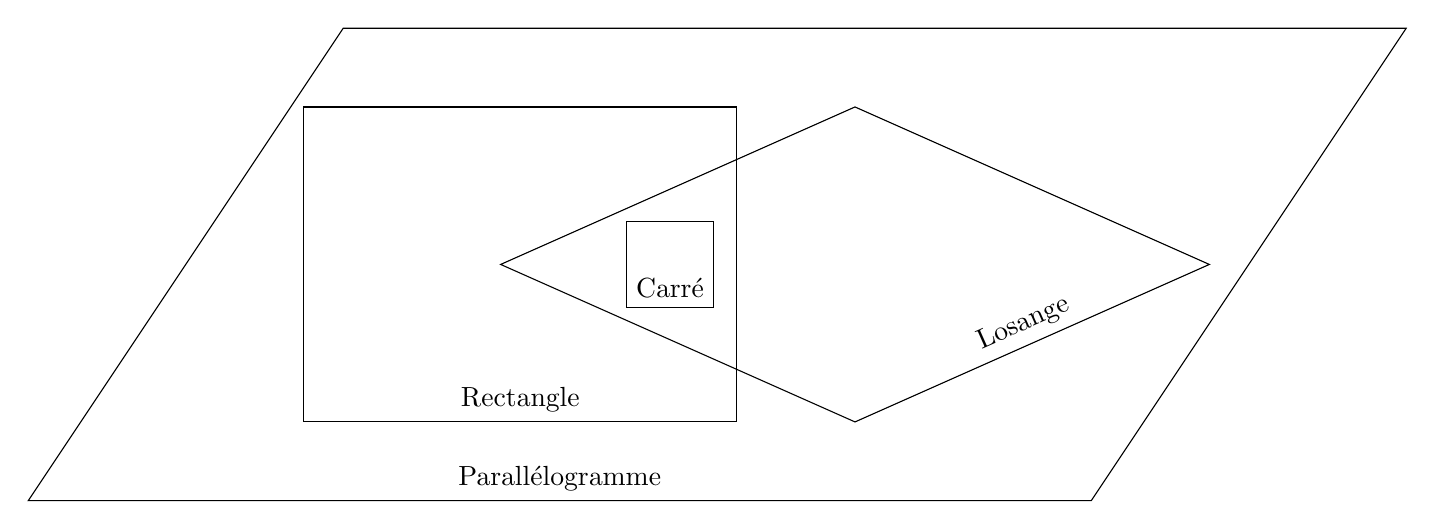
\begin{tikzpicture}
        \draw (0,0)--node [midway, above] {Parallélogramme} (13.5,0)--(17.5,6)-- (4,6)--cycle; %parallelogramme
        \draw (3.5,1)--node [midway, above] {Rectangle} (9,1)--(9,5)--(3.5,5)--cycle; %rectangle
        \draw (6,3)--(10.5,5)-- (15,3)--node [midway,above, sloped] {Losange}(10.5,1)--cycle; %losange
        \draw (7.6,2.45) -- node [midway, above] {Carré} (8.7,2.45) -- (8.7,3.55)--(7.6,3.55)-- cycle; %carré
    \end{tikzpicture}
\end{center}
